\documentclass[12pt]{article}

% Page layout
\usepackage{geometry}
\geometry{
  letterpaper,
  margin=1in
}

% Fonts and formatting
\usepackage{lmodern}
\usepackage{setspace}
\usepackage{xcolor}
\usepackage{tabularx}


% For better title control
\usepackage{titling}

\title{\vspace{2cm}
  \textbf{\Huge AstroStreet AR}\\[1em]
  \textbf{\Large Software Design Document (SDD)}\\[0.5em]
  \rule{0.8\textwidth}{0.5pt}\\[0.5em]
  \large CS 3338 -- Software Engineering Tools
}
\author{
  \large Group 2\\[0.5em]
  Royce Jamerson\\
  Khalid Jamil\\
  Michael Lieng\\
  Ricardo Ibanez
}
\date{\large December 2, 2025}

\usepackage{graphicx} % you may already have this
\usepackage{tikz}
\usetikzlibrary{arrows.meta, positioning}


\begin{document}

% ---------- Cover Page ----------
\begin{titlepage}
    \centering
    \vspace*{2cm}

    {\Huge \textbf{AstroStreet AR}\par}
    \vspace{0.8cm}
    {\Large \textbf{Software Design Document (SDD)}\par}
    \vspace{0.5cm}
    {\large Assignment 14\par}
    \vspace{0.5cm}
    {\large CS 3338 -- Software Engineering Tools\par}
    \vspace{0.5cm}
    {\large California State University, Los Angeles\par}

    \vfill

    {\large \textbf{Group 2}\par}
    \vspace{0.4cm}
    {\large Royce Jamerson\par}
    {\large Khalid Jamil\par}
    {\large Michael Lieng\par}
    {\large Ricardo Ibanez\par}

    \vfill

    {\large Date: December 2, 2025\par}

    \vspace*{1.5cm}
\end{titlepage}

% ---------- Table of Contents ----------
\pagenumbering{roman}        % Roman numerals for front matter
\setcounter{tocdepth}{2}     % Include sections and subsections
\tableofcontents
\newpage

\pagenumbering{arabic}       % Start normal page numbers for body

% ---------- SDD Sections (skeleton) ----------

% --- 1. Version Description
\section{Version Description}

This section tracks the revision history of the
\textit{AstroStreet AR} Software Design Document (SDD) for
Group 2 in CS 3338 -- Software Engineering Tools.

\begin{center}
\begin{tabularx}{\textwidth}{|c|X|c|}
\hline
\textbf{Version} & \textbf{Description} & \textbf{Date} \\
\hline
1.0 &
Initial version of the Software Design Document for
\textit{AstroStreet AR}, prepared for Assignment 14. &
December 2, 2025 \\
\hline
\end{tabularx}
\end{center}

Future revisions of this document can be recorded by adding new
rows to the table with updated version numbers, dates, and brief
descriptions of the changes.

% --- 2. Introduction
\section{Introduction}
\subsection{Purpose}

The purpose of this Software Design Document (SDD) is to describe the
overall design and internal structure of \textit{AstroStreet AR}, a
mobile augmented reality (AR) shooter game developed by Group 2 for
CS 3338 -- Software Engineering Tools at California State University,
Los Angeles.
This document translates the high-level requirements of the project into
a concrete design that can guide implementation, testing, and future
maintenance.

\subsection{System Overview}

\textit{AstroStreet AR} is a smartphone game in which players go
outside, use their phone's camera, and see virtual asteroids and alien
ships overlaid on the real world.
The player rotates their body and phone to aim and taps on the screen to
fire projectiles and destroy incoming targets.
The game tracks score, player health or shields, and increasing
difficulty as more enemies appear over time.

At a high level, the system consists of:
\begin{itemize}
    \item A mobile client that renders the AR scene, handles user input,
    manages game logic, and displays the user interface.
    \item AR services provided by the underlying platform
    (e.g., ARCore/ARKit via an engine such as Unity) to track device
    position and orientation and to overlay virtual objects on the
    camera feed.
    \item Local data storage to persist high scores and basic player
    settings on the device.
\end{itemize}

\subsection{Intended Audience}

This document is intended for:
\begin{itemize}
    \item Members of Group 2, who will use the design as a blueprint for
    implementing \textit{AstroStreet AR}.
    \item The course instructor and teaching staff, who will review the
    design as part of Assignment 14.
    \item Future developers or maintainers who may extend the game's
    features, port it to new platforms, or integrate additional
    services (such as online leaderboards).
\end{itemize}

\subsection{Document Overview}

The remainder of this SDD is organized as follows:
\begin{itemize}
    \item \textbf{System Architecture} describes the major components of
    \textit{AstroStreet AR}, their responsibilities, and how they
    interact.
    \item \textbf{User Interface} presents the planned screens and HUD
    elements, including the main menu, AR gameplay view, and score
    displays.
    \item \textbf{Database Design and Explanation} outlines the data
    structures used to store high scores and game settings, and explains
    how the application accesses this data.
    \item \textbf{Glossary} defines key technical terms and acronyms
    used throughout the document.
    \item \textbf{References} lists external resources, documentation,
    and tools consulted while designing \textit{AstroStreet AR}.
\end{itemize}

% --- 3. System Architecture
\section{System Architecture}
\subsection{Architecture Overview}

The architecture of \textit{AstroStreet AR} is organized around a
single mobile client application that runs on a smartphone and
communicates with platform-specific AR services.
Within the client, the game is decomposed into modular components
that manage AR tracking, game state, enemy behavior, player input,
user interface, and local data storage.

At a high level, the system consists of the following layers:
\begin{itemize}
    \item \textbf{Presentation Layer}: Responsible for rendering the
    camera feed, drawing virtual objects (asteroids, alien ships,
    projectiles), and displaying the heads-up display (HUD) and menus.
    \item \textbf{Game Logic Layer}: Manages the core game loop,
    including spawning enemies, updating the player state, handling
    collisions, tracking score, and determining win/lose conditions.
    \item \textbf{AR and Device Services Layer}: Interfaces with the
    underlying AR framework (e.g., ARCore/ARKit via Unity) to obtain
    camera images, device pose (position and orientation), and other
    sensor data.
    \item \textbf{Data Layer}: Handles reading and writing persistent
    data, such as high scores and basic settings, on the device.
\end{itemize}

Figure~\ref{fig:architecture} conceptually illustrates the relationships
between the major components.

\begin{figure}[h]
    \centering
    \resizebox{0.9\textwidth}{!}{%
    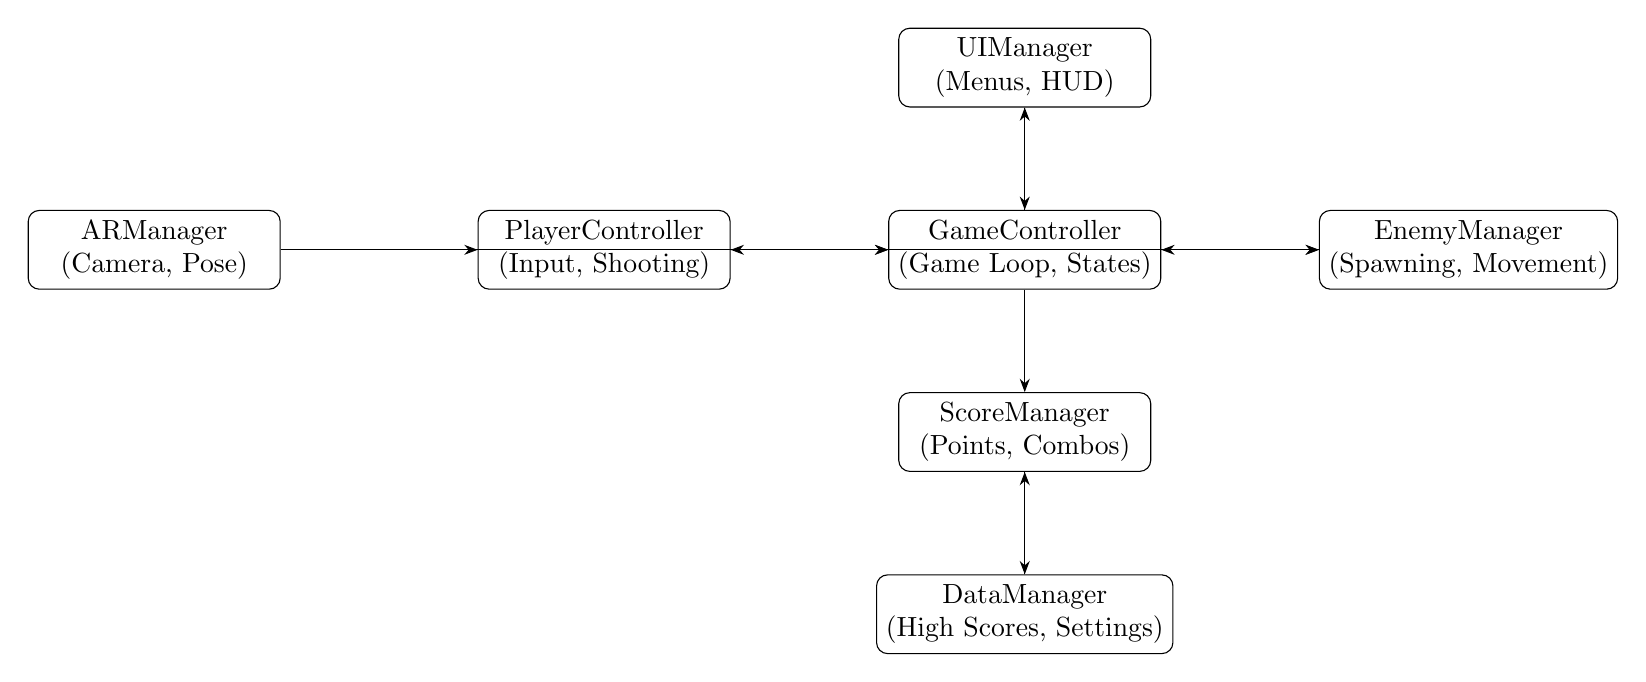
\begin{tikzpicture}[
        component/.style={
            rectangle,
            draw,
            rounded corners,
            minimum width=3.2cm,
            minimum height=1cm,
            align=center
        },
        >=Stealth,
        node distance=1.3cm and 2.0cm
    ]

    % Nodes
    \node[component] (ui) {UIManager\\(Menus, HUD)};
    \node[component, below=of ui] (game) {GameController\\(Game Loop, States)};
    \node[component, left=of game] (player) {PlayerController\\(Input, Shooting)};
    \node[component, right=of game] (enemy) {EnemyManager\\(Spawning, Movement)};
    \node[component, below=of game] (score) {ScoreManager\\(Points, Combos)};
    \node[component, below=of score] (data) {DataManager\\(High Scores, Settings)};
    \node[component, left=of player, xshift=-0.5cm] (ar) {ARManager\\(Camera, Pose)};

    % Arrows to/from GameController
    \draw[->] (ui) -- (game);
    \draw[->] (game) -- (ui);

    \draw[->] (player) -- (game);
    \draw[->] (game) -- (player);

    \draw[->] (enemy) -- (game);
    \draw[->] (game) -- (enemy);

    \draw[->] (game) -- (score);

    \draw[->] (score) -- (data);
    \draw[->] (data) -- (score);

    \draw[->] (ar) -- (game);
    \draw[->] (ar) -- (enemy);
    \draw[->] (ar) -- (player);

    \end{tikzpicture}
    }% end resizebox
    \caption{High-level component architecture of \textit{AstroStreet AR}.}
    \label{fig:architecture}
\end{figure}



\subsection{Major Components}

The main components of the client application are described below.

\subsubsection{ARManager}

The \textbf{ARManager} is responsible for:
\begin{itemize}
    \item Initializing the AR session when the game starts.
    \item Accessing the device camera feed and sensor data from the AR
    framework.
    \item Providing the current device pose (position and orientation)
    so that virtual objects can be placed consistently in the player's
    view.
\end{itemize}
Other components (such as the \textbf{GameController} and
\textbf{EnemyManager}) rely on the \textbf{ARManager} to ensure that
objects are rendered relative to the player's real-world orientation.

\subsubsection{GameController}

The \textbf{GameController} coordinates the overall game loop:
\begin{itemize}
    \item Starting and stopping gameplay sessions.
    \item Updating the game state each frame (time remaining, player
    health or shields, active enemies, and projectiles).
    \item Notifying other components when the game transitions between
    states (e.g., from ``Main Menu'' to ``In Game'' to ``Game Over'').
\end{itemize}
It serves as the central point of control, invoking the
\textbf{EnemyManager}, \textbf{PlayerController}, and
\textbf{UIManager} as needed during each update cycle.

\subsubsection{EnemyManager}

The \textbf{EnemyManager} handles all enemy-related behavior:
\begin{itemize}
    \item Spawning asteroids and alien ships according to the current
    difficulty level.
    \item Updating enemy movement and checking when enemies become too
    close to the player.
    \item Informing the \textbf{GameController} when enemies are
    destroyed or when they collide with the player.
\end{itemize}
The \textbf{EnemyManager} uses AR pose information from the
\textbf{ARManager} to decide where to place enemies in the player's
field of view.

\subsubsection{PlayerController}

The \textbf{PlayerController} interprets user input and updates the
player's actions:
\begin{itemize}
    \item Reading touch input (e.g., tapping the screen to shoot).
    \item Aligning the virtual crosshair or reticle with the player's
    current viewing direction.
    \item Requesting the creation of projectiles when the player fires
    and reporting hits back to the \textbf{GameController}.
\end{itemize}
It acts as the bridge between physical device movements/touches and
in-game actions.

\subsubsection{UIManager}

The \textbf{UIManager} manages the user interface and HUD:
\begin{itemize}
    \item Displaying the main menu, pause menu, and game over screen.
    \item Rendering HUD elements during gameplay, such as the score,
    health or shield bar, time remaining, and any active power-ups.
    \item Receiving navigation commands from the user (e.g., starting a
    new game, returning to the main menu).
\end{itemize}
The \textbf{UIManager} communicates with the \textbf{GameController}
and \textbf{ScoreManager} to update visual information.

\subsubsection{ScoreManager}

The \textbf{ScoreManager} tracks and updates the player's score:
\begin{itemize}
    \item Awarding points when enemies are destroyed.
    \item Applying score multipliers or bonuses for streaks.
    \item Exposing the current score to the \textbf{UIManager} for
    display during gameplay.
\end{itemize}
At the end of a game session, the \textbf{ScoreManager} collaborates
with the \textbf{DataManager} to save high scores.

\subsubsection{DataManager}

The \textbf{DataManager} is responsible for:
\begin{itemize}
    \item Persisting high scores and basic settings (such as sound
    preferences and control sensitivity) to local storage on the
    device.
    \item Loading saved data when the application starts.
    \item Providing a simple interface for other components to read and
    write data without dealing directly with the storage mechanism.
\end{itemize}

\subsection{Component Interactions}

During a typical gameplay session, the components interact as follows:
\begin{enumerate}
    \item The user selects ``Start Game'' from the main menu.
          The \textbf{UIManager} notifies the \textbf{GameController}
          to begin a new session.
    \item The \textbf{GameController} initializes the game state and
          requests the \textbf{ARManager} to start the AR session.
    \item The \textbf{EnemyManager} begins spawning enemies in positions
          derived from the AR pose provided by the \textbf{ARManager}.
    \item Each frame, the \textbf{PlayerController} reads user input
          (screen taps) and creates projectiles along the player's
          current viewing direction.
    \item The \textbf{GameController} updates all active entities,
          checks for collisions between projectiles and enemies, and
          adjusts the player's health or shields if enemies get too
          close.
    \item The \textbf{ScoreManager} updates the score when enemies are
          destroyed, and the \textbf{UIManager} refreshes the HUD to
          show the latest score and health values.
    \item When the game ends (e.g., the player's health reaches zero),
          the \textbf{GameController} notifies the \textbf{ScoreManager}
          and \textbf{DataManager} to save the final score, then
          instructs the \textbf{UIManager} to display the game over
          screen.
\end{enumerate}

This modular architecture is intended to keep responsibilities clearly
separated, making the system easier to implement, test, and extend with
future features such as additional enemy types, power-ups, or online
leaderboards.

% --- 4. User Interface 
\section{User Interface}

\subsection{Overview}

The user interface (UI) of \textit{AstroStreet AR} is designed to be
simple and usable outdoors while the player is holding a smartphone.
Navigation is primarily tap-based, and the most important information
(score, health, and basic controls) is always visible during gameplay.

The main UI elements include:
\begin{itemize}
    \item A \textbf{main menu} for starting the game and accessing other
    screens.
    \item An \textbf{AR gameplay view} that overlays enemies and HUD
    elements on top of the camera feed.
    \item A \textbf{pause menu} for temporarily stopping gameplay.
    \item A \textbf{game over screen} that summarizes the player's
    performance.
    \item A \textbf{high scores} screen.
    \item A \textbf{settings} screen for basic configuration options.
\end{itemize}

\subsection{Main Menu}

When the application launches, the user is shown the main menu screen.
This screen contains:
\begin{itemize}
    \item The game title: \textbf{AstroStreet AR}.
    \item A brief subtitle or tagline (e.g., ``Aim at the sky and blast
    incoming asteroids!'').
    \item A set of buttons:
    \begin{itemize}
        \item \textbf{Start Game} -- begins a new AR gameplay session.
        \item \textbf{High Scores} -- opens the high scores screen.
        \item \textbf{Settings} -- opens the settings screen.
        \item \textbf{Exit} (optional on platforms that support it) --
        closes the application.
    \end{itemize}
\end{itemize}

The main menu is displayed on top of a static or subtly animated
background image related to outer space or the night sky.
From this screen, the player can reach all other major UI flows.

\subsection{AR Gameplay Screen}

The AR gameplay screen is the core of the user experience.
It uses the device camera feed as the background and overlays virtual
game elements on top.

The key elements of this screen are:
\begin{itemize}
    \item \textbf{Camera View}: The live camera feed fills the entire
    screen to show the player's real-world surroundings.
    \item \textbf{Crosshair or Reticle}: A small graphical reticle is
    centered on the screen and indicates where the player's shots are
    aimed.
    \item \textbf{Score Display}: The current score is shown in the
    upper-left corner of the screen.
    \item \textbf{Health or Shield Bar}: The player's remaining health
    or shield is represented as a bar or set of segments in the
    upper-right corner.
    \item \textbf{Timer} (if used): If the game mode uses a time limit,
    the remaining time is displayed near the top of the screen.
    \item \textbf{Pause Button}: A small pause icon appears in one
    corner (e.g., top-right), allowing the user to open the pause menu.
\end{itemize}

To interact with this screen, the user:
\begin{itemize}
    \item Physically rotates or tilts the phone to aim the reticle at
    enemies that are rendered in the AR view.
    \item Taps the screen to fire projectiles in the direction of the
    reticle.
\end{itemize}

Enemies (asteroids and alien ships), projectiles, explosions, and
power-ups are all rendered as virtual objects anchored in the AR scene.

\subsection{Pause Menu}

The pause menu appears when the user taps the pause button during
gameplay.
When the game is paused, the AR scene is dimmed or frozen, and a small
overlay panel is shown with the following options:
\begin{itemize}
    \item \textbf{Resume} -- returns to the AR gameplay screen and
    continues the session.
    \item \textbf{Settings} -- opens a subset of settings (for example,
    sound on/off and sensitivity) without leaving the session.
    \item \textbf{Quit to Main Menu} -- ends the current game and
    returns to the main menu.
\end{itemize}

\subsection{Game Over Screen}

When the player's health reaches zero or the game session ends for
another reason (such as a time limit), the game over screen is shown.

This screen contains:
\begin{itemize}
    \item A prominent ``Game Over'' title.
    \item The player's final score.
    \item An indication if a new high score was achieved.
    \item Buttons for:
    \begin{itemize}
        \item \textbf{Play Again} -- start a new game session.
        \item \textbf{Return to Main Menu} -- go back to the main menu.
    \end{itemize}
\end{itemize}

\subsection{High Scores Screen}

The high scores screen displays a list of the top scores recorded on
the device.
A simple layout might include:
\begin{itemize}
    \item A title such as ``High Scores''.
    \item A table or vertical list showing rank, score value, and date
    achieved.
    \item A button to return to the main menu.
\end{itemize}

\subsection{Settings Screen}

The settings screen allows the user to adjust basic configuration
options for \textit{AstroStreet AR}.
Possible settings include:
\begin{itemize}
    \item \textbf{Sound}: toggle sound effects on or off.
    \item \textbf{Control Sensitivity}: adjust how quickly the reticle
    responds to device movement.
    \item \textbf{Brightness or UI Contrast}: optional adjustments to
    help make the HUD more readable outdoors.
\end{itemize}

The settings screen is accessible from both the main menu and the pause
menu, and includes a button to return to the previous screen.

Overall, the user interface is designed to minimize on-screen clutter so
that players can clearly see both the real world and the virtual
objects they are interacting with while playing \textit{AstroStreet AR}.

% --- 5. Data Design and Explanation
\section{Database Design and Explanation}

\subsection{Overview}

\textit{AstroStreet AR} uses a small amount of persistent data to store
player high scores and basic configuration settings.
In a mobile implementation, this data can be stored using a lightweight
mechanism such as a local database (e.g., SQLite), key--value storage,
or the game engine's built-in persistence system.
This section describes the logical database design that the
\textbf{DataManager} component works with, independent of the specific
storage technology.

The primary data entities are:
\begin{itemize}
    \item \textbf{HighScore}: represents a single recorded high score.
    \item \textbf{Setting}: represents a user-adjustable configuration,
    such as sound or control sensitivity.
\end{itemize}

\subsection{HighScore Entity}

The \textbf{HighScore} entity stores the results of completed game
sessions.
Each record corresponds to one high score achieved by the player.

\begin{center}
\begin{tabularx}{\textwidth}{|c|c|X|}
\hline
\textbf{Field} & \textbf{Type} & \textbf{Description} \\
\hline
HighScoreID & Integer & Unique identifier for the high score entry. \\
\hline
PlayerName & Text & Optional name or initials provided by the player
(e.g., ``RJ''). \\
\hline
Score & Integer & Final score achieved at the end of a game session. \\
\hline
DateAchieved & DateTime & Date and time when the score was recorded. \\
\hline
\end{tabularx}
\end{center}

In a simple single-player implementation, \texttt{PlayerName} can be
optional or default to a generic value (such as ``Player'').
The \textbf{DataManager} is responsible for:
\begin{itemize}
    \item Inserting a new \textbf{HighScore} record when a game ends.
    \item Retrieving the top \textit{N} scores ordered by \texttt{Score}
    (and optionally by \texttt{DateAchieved}) for display on the
    High Scores screen.
    \item Deleting or pruning old scores if a maximum number of
    stored records is desired.
\end{itemize}

\subsection{Setting Entity}

The \textbf{Setting} entity stores simple key--value pairs that
represent user preferences for the game.

\begin{center}
\begin{tabularx}{\textwidth}{|c|c|X|}
\hline
\textbf{Field} & \textbf{Type} & \textbf{Description} \\
\hline
SettingKey & Text & Unique key name for the setting
(e.g., \texttt{``soundEnabled''}, \texttt{``sensitivity''}). \\
\hline
SettingValue & Text & String representation of the value
(e.g., \texttt{``true''}, \texttt{``0.8''}).
This can be parsed into the appropriate type (boolean, number, etc.)
by the \textbf{DataManager}. \\
\hline
\end{tabularx}
\end{center}

Examples of settings that might be stored include:
\begin{itemize}
    \item \texttt{soundEnabled}: whether sound effects are on or off.
    \item \texttt{sensitivity}: a numeric value controlling how quickly
    the reticle responds to device movement.
    \item \texttt{uiBrightness}: an optional value controlling HUD
    brightness or contrast.
\end{itemize}

The \textbf{DataManager} provides simple operations to:
\begin{itemize}
    \item Read a setting by its \texttt{SettingKey}, returning a default
    value if it has not been set yet.
    \item Write or update a setting when the user changes options in the
    Settings screen.
\end{itemize}

\subsection{Relationships and Data Flow}

The logical relationship between the entities is straightforward:
\begin{itemize}
    \item Each \textbf{HighScore} record is independent and does not
    reference other records.
    \item Each \textbf{Setting} record is identified by a unique
    \texttt{SettingKey}, forming a key--value store.
\end{itemize}

During normal operation:
\begin{enumerate}
    \item At application startup, the \textbf{DataManager} loads
          existing \textbf{Setting} records and applies them to the
          game (for example, enabling or disabling sound).
    \item When the user finishes a game, the \textbf{ScoreManager}
          passes the final score to the \textbf{DataManager}, which
          creates a new \textbf{HighScore} record with the score and
          current date.
    \item When the user opens the High Scores screen, the
          \textbf{UIManager} requests the list of top scores from the
          \textbf{DataManager} and displays them.
    \item When the user changes a setting in the Settings screen, the
          \textbf{UIManager} calls the \textbf{DataManager} to update
          the corresponding \textbf{Setting} record.
\end{enumerate}

This simple database design is sufficient for the current scope of
\textit{AstroStreet AR} and can be extended in the future (for example,
to support multiple named players or to synchronize scores with an
online leaderboard) without significantly changing the rest of the
system architecture.


% --- 6. Glossary
\section{Glossary}

This section defines key terms and acronyms used throughout the
\textit{AstroStreet AR} Software Design Document.

\begin{center}
\begin{tabularx}{\textwidth}{|c|X|}
\hline
\textbf{Term} & \textbf{Definition} \\
\hline
AR (Augmented Reality) &
A technology that overlays virtual objects (such as asteroids and
alien ships) onto a live view of the real world, typically using a
camera and device sensors. \\
\hline
UI (User Interface) &
The visual elements and interactive controls that the player uses to
navigate the application, such as buttons, menus, and icons. \\
\hline
HUD (Heads-Up Display) &
On-screen information shown during gameplay, including the score,
health or shield bar, timer, and other status indicators. \\
\hline
FPS (Frames Per Second) &
The number of times per second that the game updates and redraws the
screen; higher FPS generally results in smoother gameplay. \\
\hline
API (Application Programming Interface) &
A defined set of functions or endpoints that one software component
can use to communicate with another, such as an AR framework or a
web service. \\
\hline
ARCore / ARKit &
Platform-specific AR frameworks provided by Google (ARCore) and Apple
(ARKit) that supply camera images, device pose, and tracking
capabilities to mobile applications. \\
\hline
Component &
A logical part of the system with a specific responsibility, such as
\textbf{GameController}, \textbf{EnemyManager}, or
\textbf{DataManager}. \\
\hline
Entity &
A logical representation of a data object stored by the system, such
as a \textbf{HighScore} or \textbf{Setting}. \\
\hline
Game Session &
A single continuous playthrough that starts when the player begins a
game and ends when the player loses, quits, or returns to the main
menu. \\
\hline
Persistent Data &
Information that is saved to storage so that it remains available
after the application is closed, such as high scores and user
settings. \\
\hline
\end{tabularx}
\end{center}


% --- 7. References
\section{References}

This section lists external resources, tools, and documentation that
inspired or informed the design of \textit{AstroStreet AR}.

\begin{thebibliography}{9}

\bibitem{unity-ar}
Unity Technologies,
\textit{Unity Manual: AR Foundation}.
Available at: https://docs.unity3d.com/Packages/com.unity.xr.arfoundation

\bibitem{google-arcore}
Google,
\textit{ARCore Developer Guide}.
Available at: https://developers.google.com/ar

\bibitem{apple-arkit}
Apple Inc.,
\textit{ARKit Overview}.
Available at: https://developer.apple.com/augmented-reality

\bibitem{game-architecture}
Jason Gregory,
\textit{Game Engine Architecture}.
A K Peters/CRC Press, 2nd edition, 2014.

\bibitem{latex-guide}
Leslie Lamport,
\textit{\LaTeX: A Document Preparation System}.
Addison-Wesley, 2nd edition, 1994.

\end{thebibliography}


\end{document}
